You can now enter data for the references you entered during specification.

\begin{enumerate}
\item In the \gdtestcaseeditor{}, single-click on the \bxname{First Test} node. 
\item In the \gddatasetsview{}, select \bxcaption{add}. 
\item In the row which appears, enter \bxshell{3} in the  field for 
\bxcaption{V1}, \bxshell{3} in the field for \bxcaption{V2} and \bxshell{6}
in the field for \bxcaption{RES}.  
\item Select  \bxcaption{Add} again. In the second row which appears, enter:
\\
\\
\begin{tabular}{|p{0.2\bxpicwidth}|p{0.2\bxpicwidth}|p{0.2\bxpicwidth}|}\hline
 \textbf{V1}& \textbf{V2}& \textbf{RES} \\ \hline
 17& 4& 21 \\ \hline
\end{tabular}

\item Repeat the above step once more for a third row, with the values:
\\
\\
\begin{tabular}{|p{0.2\bxpicwidth}|p{0.2\bxpicwidth}|p{0.2\bxpicwidth}|}\hline
 \textbf{V1}& \textbf{V2}& \textbf{RES} \\ \hline
 40& 2& 42 \\ \hline
\end{tabular}
\item Your \gddatasetsview{} should now have three data sets (\bxfigref{TutDataSets}).
\begin{figure}[h]
\begin{center}
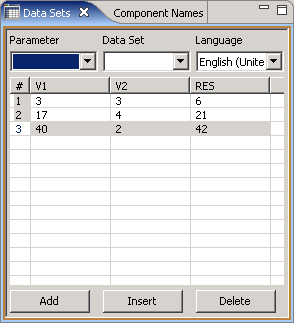
\includegraphics{Tutorials/PS/TutDataSets}
\caption{The \gddatasetsview{}}
\label{TutDataSets}
\end{center}
\end{figure}

\item Press \bxcaption{save}.
\item These data will be used whenever you use this \gdcase{}. You can overwrite them when you reuse the \gdcase{} if you want to.  
\end{enumerate}
